\chapter{Definitions, Syntax, and the Cycles Invariant}



\section{Graphs}

This report describes undirected, unlabeled graphs with no self-loops or multi-edges.
Such graphs are represented by an \emph{adjacency matrix}: a square, symmetric, binary matrix with zeros along the diagonal.
We will use $G$ to refer to a graph, and $A$ to refer to an adjacency matrix of the graph.
When we use $A$, it will not refer to a specific adjacency matrix, as most graphs can be represented by many matrices.

We will refer to the set of vertices of a graph as $V(G)$, and the set of edges of a graph as $E(V)$.
Graphs have $N$ vertices and $M$ edges where $N \in [0, \infty)$ and $M \in [0, E_{max}]$ where ${E_{max}} = \frac{1}{2}(N)(N-1)$.
When discussing specific edges, tuples are symmetric: $(v_1, v_2) = (v_2, v_1)$.

A graph's \emph{complement} or \emph{inverse} is a new graph over the same set of vertices, but where adjacency and non-adjacency are inverted.
In formal terms, the graph $\xoverline{G}$ is $G$'s inverse if $V(\xoverline{G}) = V(G)$ and $(v_1, v_2) \in E(\xoverline{G}) \leftrightarrow (v_1, v_2) \notin E(G)$.

The complete graph over $N$ vertices is $K_N$. 
The cycle graph over $N$ vertices is $C_N$.
The star graph over $N$ vertices is $S_N$.
The empty graph over $N$ vertices is $E_N$.



\section{Labeling and Representing Graphs}

A labeling of a graph is a bijection which maps each vertex of $V(G)$ to an integer in the range $[1, N]$.
For every possible labeling of a graph, there is a natural adjacency matrix which represents it, namely the matrix where the $i$\ts{th} labeled vertex is represented by the $i$\ts{th} column and row of the matrix.
The number of distinct labelings of a graph and the number of distinct matrices which represent that graph are equivalent.
A graph can have as many as $V!$ labelings, or can have as few as $1$ (consider $K_N$).

An important distinction in this report is on the \emph{representation} of graphs.
Most graphs can be represented by several distinct adjacency matrices, but a change to representation does not change the fundamental structure of the graph that the matrices represent.
Different representations of graphs are akin to different labelings of the graph: neither mutate structure, and neither should change the results of our algorithms.
When we discuss a set of graphs, or an algorithm over graphs, we will be treating graphs as objects which denote structure, and will in every way be blind to their representation.
When we refer to a graph, we are referring to all of its representations.
When we intend to discuss a graph within some physical reality of its representation (for example, when determining whether two given adjacency matrices refer to the same graph) we will use the term \emph{graph instance} to denote that difference.
This is an `algebraic' understanding of the structure of graphs, not a semantic choice. 
It will have important implications throughout this report, particularly around ideas of random graph models.

When we are discussing the set of all graphs as algebraic objects, we will use the notation $G_{Alg}$.
When we are discussing the set of all graph instances, we will use the notation $G_{Inst}$.
To start thinking critically about this distinction, always remember that:
$$|G_{Alg}| <<< |G_{Inst}| = 2^{E_{max}}$$
but since the number of representations of a given graph is limited by its number of labelings that:
$$|G_{Alg}| * N! > | G_{Inst} | =  2^{E_{max}}$$

Finally, we will talk about the number of distinct matrices that describe isomorphic graph instances as being the `number of representations' of the graph, or $M_{Reps}(G) \in [1, N!]$.
Note that  $M_{Reps}(G)$ is related to the differentiation we made between the set of all graphs ($G_{Alg}$) and the set of all graph instances ($G_{Inst}$).

\subsection{Graph6 Encoding of Graphs}

For this project, we frequently will use graph6 notation to encode a graph as a succinct string.
This is an encoding of the adjacency matrix as described through the formal specification (http://users.cecs.anu.edu.au/~bdm/data/formats.txt).
Basically, we take the upper half of the adjacency matrix (not including the zeroed-out diagonal), as a bit-string, then compress that bit-string using UTF-8 character encoding.
I optimized this code (preallocation, bit shifting, etc) in all of the languages I used, because when non-optimized, it can contribute to runtime in a non-negligible way.

\subsection{Counting Graphs over N Vertices}

The number of undirected, non-looped graphs over N vertices is an open question in computational theory.
The first few values of this sequence were well known, however no closed form has been proven to successfully list the numbers of graphs of a given size.
A large number of theoreticians have come up with proposed closed forms with associated margins of error, but all small values have been agreed upon.
The values in this sequence grow exponentially, but to give you an idea of how rapidly, the first twelve values are shown:

$$1\,\; \;1\, \;\;2\, \;\;4\, \;\;11\, \;\;34\, \;\;156\, \;\;1044\,\; 12346\,\;\; 274668\, \;\;12005168\, \;\;1018997864$$

Thus, when we describe (as we will throughout this project) the computational difficulty of going, say, from calculating a metric over all graphs on 10 to 11 vertices, remember that is about a 60-fold increase in the size of the examined set, not even beginning to grapple with the time complexity increase that an increase in $N$ has on the running time of the algorithm.
The values that I use for this thesis come directly from the Online Encyclopedia of Integer Sequences, which gives values up to graphs with 50 vertices.
As a side note: OEIS is probably one of my favorite things that exists.
It astounds me how good it is picking out the exact sequence you are looking for, regardless of whether it is shifted by a few places, might have missing gap, etc.
A well cooked example of the beautiful hyper-connected and data-driven world we live in.

\subsection{Counting Graphs over N Vertices and M Edges}

The number of graphs with a given number of nodes (N), has an internal distribution: the number of edges in each of the graphs.
It turns out that this is an approximately normal distribution, which is (as we would anticipate) centered at $\frac{E_{Max}}{2}$. 
To see how this distribution changes over various values of N, we can normalize our notion of edges to one of connectivity:
we will divide the number of edges by the number of possible edges (transforming an integer range $[0, E_{max}]$ to a fractional range $[0, 1]$.

This enables us to see how the distribution changes over multiple values of N.
In figure \ref{fig:ngraphs} we make clear this connection by normalizing the distributions so that they are comparable (i.e. making the areas under each curve exactly one by dividing each by the total number of graphs associated with the value of N), we are able to capture the way that the distribution of graph connectivity changes for varying values of N and M.

\begin{figure}[h]
\label{fig:ngraphs}
\caption{\emph{Number of Graphs over N vertices with varying Connectivity}}
\centering
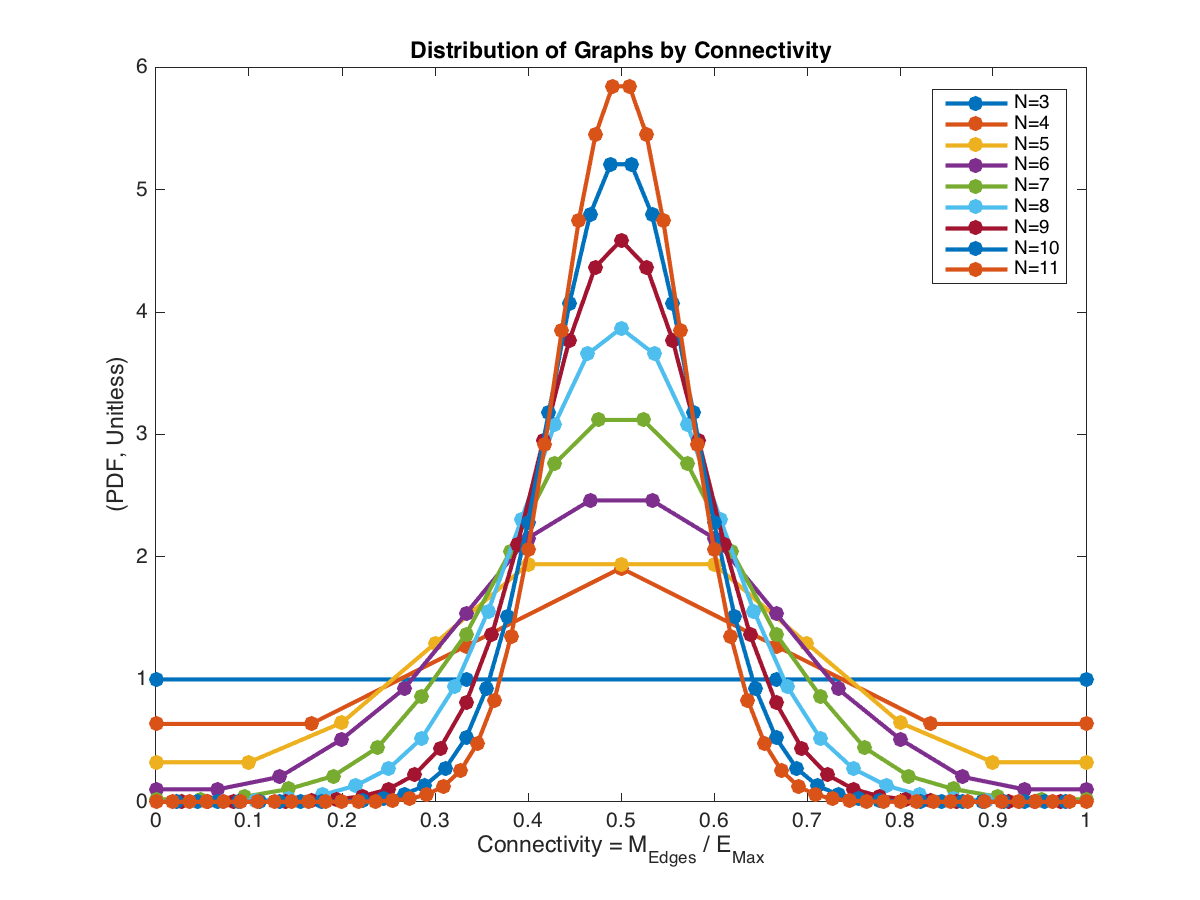
\includegraphics[width=\textwidth]{pdfs3thru11}
\end{figure}

When normalized in this manner, it becomes immediately clear that:
\begin{itemize}
\item{Each of these distributions is normaly distributed}
\item{The distributions share peaks (as we expect them to) at 1/2}
\item{The standard deviation of each of these distributions is decreasing as N increases}
\end{itemize}

To formalize these three observations, I first ran normality tests, which passed at the most strict levels possible for $N \geq 8$, and which were slightly less performant for smaller values of N (which makes sense, as we simply have fewer discrete bins on our x-axis in which to place observations, which are also many fewer in number).
Secondly, I verified our thinking on the co-modality trivially: we know that if two graphs are non-isomorphic, then their inverses are non-isomorphic.
Thus, our distribution must be symmetric about the half-connectivity point.
Thirdly, we can formalize this by fitting a normal distribution to each of the observed relationships between population proportion and connectivity (allowing only sigma to vary) and come up with precise estimates for the normal fits for these distributions for $N \geq 5$.
I opted not to use the fitted sigmas for $N < 5$, as the roughness of our data for those values meant that less than 90\% of the variation in those observations was attributable to the normality.
The results are shown below in figure \ref{fig:decreasingsigma}, and there is a clear downward trend in sigma, which roughly follows a power curve which asymptotes to zero:

\begin{figure}[h]
\label{fig:decreasingsigma}
\caption{\emph{Standard Deviation Fit to Distribution of Number of Edges for Graphs over N Vertices}}
\centering
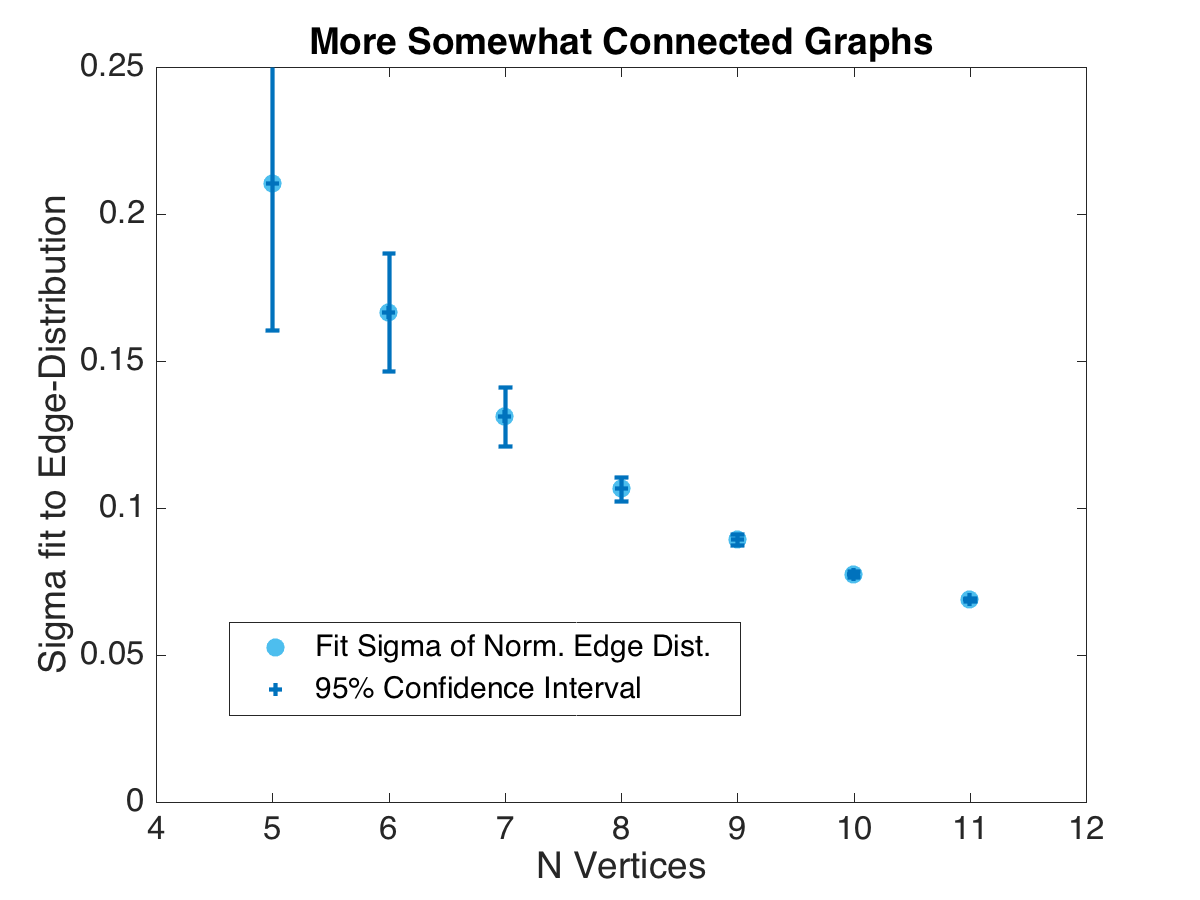
\includegraphics[width=\textwidth]{decreasingsigma}
\end{figure}

This establishes an important relationship: most graphs are `somewhat connected', neither sparse nor dense, with an increasing probability that they lie in the middle of the connectivity distribution.
In fact, it appears that as N increases, sigma decreases, and we can conclude that the larger the value of N, the fewer and fewer graphs (as a proportion of the global set) are sparse or dense.

\section{Graph Isomorphism and Automorphism}

Two graph instances $G$ and $H$ are \emph{isomorphic} if there exists a mapping $M$ between $V(G)$ and $V(H)$ such that $$\forall_{a, b \in V(G)} (a, b) \in E(G) \leftrightarrow (M(a), M(b)) \in E(H)$$

If an isomorphism exists between two graph instances, then the two instances represent the same graph; they have the same structure.
An isomorphism preserves all adjacencies and all non-adjacencies, and the existence of an isomorphism between instances proves that they are the same graph.
It may be possible for multiple isomorphisms to exist between two graph instances, but we are generally only concerned with the existence of such a mapping.
We will use the notation $Iso(G, H)$ to be shorthand for a boolean predicate describing the existence of such a mapping.

The question of whether or not graph isomorphism as a decision problem (GI) can be computed in polynomial time is an open question in theoretical computer science.
The advancement of Babai in November of 2015 proved that GI is computable in quasi-polynomial time, though no convincing arguments have placed it in NP-complete nor in P.

An \emph{automorphism} is a mapping of the set of vertices of a graph onto itself ($V(G)$ to $V(G)$) which preserves adjacency and non-adjacency.
If an automorphism $M$ maps every element of $V(G)$ to itself, the automorphism is called the \emph{trivial automorphism}.
Though it will be taken as granted, the set of all valid automorphisms for a graph G forms a group.
This group has at least one element (the identity element as the identity automorphism), but may have as many as $N!$ elements.
This group will be referred to as $Aut(G)$, and the operation over the group is understood to be the \emph{followed by} operation.



\section{Graph Invariants}
A \emph{graph invariant} is an ordered property calculated over a graph which remains the same irrespective of the representation or labeling of the graph.
More specifically, an algorithm or property is a graph invariant only if it produces output which is stable across all instances of the same graph.
A graph invariant $Inv(G)$ can allow us to conclude that two graph instances $(G_1, G_2)$ are \emph{not} isomorphic if $Inv(G_1) \neq Inv(G_2)$.
However, it is distinctly limited, in that the converse does not nescesarily hold (i.e. it is possible for non-isomorphic graph instances to share a value for a graph invariant).


\subsection{Discriminatory Power}
A graph invariant is \emph{discriminating} if it can, with a certain probability, distinguish two non-isomorphic graphs as non-isomorphic.
For example, an example of a graph invariant that is not very discriminatory is the vertex count of a graph.
Two graphs are certainly not isomorphic if they differ in their vertex count, however, many graphs which are not isomorphic do have the same vertex count.
In contrast, the chromatic polynomial of a graph is a highly discriminatory graph invariant, as the odds of having two non-isomorphic graph instances agree on their chromatic polynomial is relatively low.

To formalize this notion, we will discuss discriminatory power with a specific probabilistic meaning.
A graph invariant $Inv$ discriminates at a level $\alpha$ for $N$ vertices and $M$ edges if selecting two graphs $G$ and $H$ at random from some random graph generator:
$$P \big[ Inv(G) = Inv(H) \wedge \neg Iso(G, H) \big] \, \leq \, \alpha$$
What we will find is that we can frequently discuss alpha as a function of $M$ and $N$.
Later in this report we will discuss how $\alpha$ fits in to a natural definition of a false positive an uncertain test without a false negative rate ($\beta = 0$).



\section{Vertex Invariants}


\subsection{Vertex Similarity}
Two vertices are \emph{similar} if there exists a mapping in the automorphism group $Aut(G)$ such that the mapping maps one vertex to the other.
Similarity is a transitive and commutative property.
The vertex set $V(G)$ can be divided up into between 1 and N similar vertex sets, such that all of the vertices in each set are similar, and no two sets contains similar vertices.
A discussion of these \emph{similar vertex sets} (or SVSs) will be the primary focus of chapter three.

A graph (or subset of the vertices of a graph) is called \emph{perfectly similar} or \emph{perfectly automorphic} if, for every pair of vertices, there exists an automorphic mapping which maps one of the vertices to the other.
This is not suggesting that every mapping of the graph is an automorphism (as is only the case in $K_n$ and $\xoverline{K_n}$), but rather that any initial choice of pairing within a mapping is valid, even if it limits further choices.
For example, $C_n$ is a perfectly similar graph, as is Peterson's graph.


\subsection{Vertex Invariants}
\emph{Vertex invariants} are numerical properties that we  calculate over a specific vertex within a graph which identifies potentially similar vertex pairs.
Similar vertices within a graph agree on all vertex invariants.
However, like graph invariants, vertex invariants can only eliminate the possibility for vertex similarity, they are not sufficient to prove similarity.

Vertex invariants make the computation of graph isomorphism between two graphs markedly easier. 
Whereas a graph invariant can tell us about whether or not graph instances as a whole might be alike, it does nothing to suggest a proposed mapping between the vertices of the two graph instances.
In contrast, a vertex invariant identifies potentially similar vertices not only within a graph, but also between graph instances.
A \emph{perfect} vertex invariant is one for which agreement on the value of the invariant is equivalent to establishing the existence of an automorphism that maps one vertex to the other.

A question discussed later in this report will be about the theoretical implications of a hypothetical perfectly discriminatory vertex invariant, and a proposed invariant that haven't been found to be imperfect.



\section{Cycles Invariant}
The focus of this report is an invariant which can function as an invariant over graphs or their vertices.
It is called the `Cycles' invariant, but is sometimes referred to as the `Paths' Invariant in cases where cycle has other connotations.
In either case, we will consistently capitalize to distinguish the invariant from its other denotations.

Our definition of cycles counts ones which repeat vertices and edges, and ones which can pass back through their place of origin.
We are counting cycles which are directional, so $ABCA$ and $ACBA$ are distinct cycles.

Note that cycles (as a function and vertex invariant) is a property of a graph instance, only through sorting can we make it into a graph invariant.


\subsection{Cycles as a Function}

The $Cycles(A, p, v)$ invariant counts the number of closed paths of length $p$ that pass through a given vertex, $v$. 
This information can be easily computed using $A$. 
Just as the entries of $A^1$ represent the existence of paths of length 1 between two vertices (edges), the entries of $A^p$ represent the number of paths of length $p$ between any two vertices (by examining the row and column corresponding to two vertices).
Thus, to find the number of closed paths of length $p$ that contain a given vertex $v$, we simply need to calculate: 
$$Cycles(A, p, v) = A^p[v, v]$$
Where $v$ is being used interchangeably here with its represented position within the adjacency matrix. 
Thus, calculating a specific value of $Cycles(A, p, v)$ can occur in the time it takes to exponentiate $A$ to the power $p$.

Though it is a well known result that matrix multiplication can be done in faster than $O(n^3)$ time, we will be using the na\"{i}ve assumption that matrix multiplication runs in $O(n^3)$ in order to make the computational complexity calculations more accessible.  
Under that simplifying assumption, it is clear that calculating $Cycles(A, p, v)$ will occur in $O(p N^3)$ time, but we can request as many values of $v$ and $p_i < p$ `for free' after a single calculation for $A$ and $p$.


\subsection{Cycles as a Vertex Invariant}

Cycles as a vertex invariant describes a vector of length $P$, where the $p$th entry is the number of closed cycles of length $p$ which pass through the vertex being described.

If a vertex is the $i$th row/column of an adjacency matrix $A$, then the cycles invariant for the vertex is the successive values of 
$$Cycles(A, v_i) = [c_1, c_2, ... c_N] \text{such that} c_p = Cycles(A, v_i, p) = A^p[i,i]$$
for each of the values of $p$, forming a vector of length $P$.

The vector generated by this computation is a way of describing the local graph around the vertex $v_i$.
We can consider many ways in which Cycles reflects a `reverberation' about the local neighborhood of a vertex, and provides a noisy invariant, which is useful for distinguishing between vertices in a graph. 
It will be discussed why later, but we will prove that $P$ will always be strictly less than $N$, and that further values of computation are not useful, as they cannot provide additional layers of differentiation between graphs or their vertices.


\subsection{Cycles as a Graph Invariant}

Extending this vertex invariant to be a graph invariant requires little imagination. 
We simply calculate the Cycles vertex invariant for every one of the vertices of the graph, and are given back $N$ vectors of length $P$.
We then sort the resultant vectors lexicographically, and arrange them in a $N \times P$ matrix.
This matrix is a comparable object which is invariant to changes in labeling or representation of $G$.

Thus, paths as a graph invariant takes fewer inputs: Cycles(A, P).

Since vectors are comparable in linear time, we can sort them in log-quadratic time.
This does not change the asymptotic nature of our running time.

Cycles(A, P) is invariant to changes in vertex relabeling or adjacency matrix ordering.
A skeptical reader should convince themselves that this holds true, even when two of the vectors to be sorted are identical, the resulting $Paths$ object is valid and deterministically constructed from the graph.
The specific running time of calculating and comparing the $Cycles$ functions and object is not the primary aim of this report, but there are clever methodologies that I have used to reduce the running time beyond these na\"{i}ve estimates.
Most notably, we can significantly improve upon the average case time complexity by using delayed evaluation techniques, and can improve overall running time by multi-threading the calculations across multiple cores or GPUs.

\subsection{A Brief Example}

The best way to establish intuition and understanding of the cycles invariant is to show its values on a sample graph.
In figure \ref{fig:cyclesdemograph}, we see an example graph (in graph6 format: I@QKj?]]O), which has multiple automorphisms.
The graph has been arranged to be aesthetically appealing and to make the automorphisms clear.

In figure \ref{fig:cyclesdemocycles} below, we also see the cycles matrix for the graph.
The rows represent the individual vertex invariants associated with each value of cycles.
The columns represent the length of the cycles being considered.
The reader should trace out the number of cycles for themselves (for small values of $p$) to see the connection, and understand how this function is translated to a vertex invariant, and then to a graph invariant (the full matrix).

\begin{figure}[h]
\label{fig:cyclesdemograph}
\caption{\emph{A Small Graph} - A labeling of the vertices is provided to correspond to the labeling of figure \ref{fig:cyclesdemocycles}. This graph (like all of the ones we are describing) is unlabeled, undirected, and loop-less.}
\centering
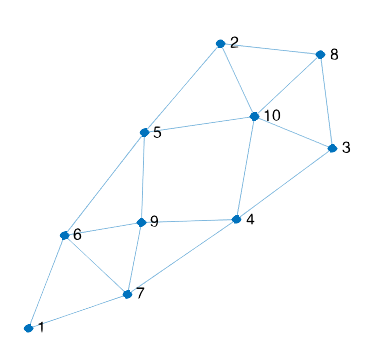
\includegraphics[width=.5\textwidth]{cyclesdemograph}
\end{figure}

\begin{figure}[h]
\label{fig:cyclesdemocycles}
\caption{\emph{A Cycles Invariant Matrix} - The color coding corresponds to the numbers, and purely serve to give a visual differentiation between different integer values.  We can see that many of the pairs of vertices in this graph share their values of the cycles invariant through them.}
\centering
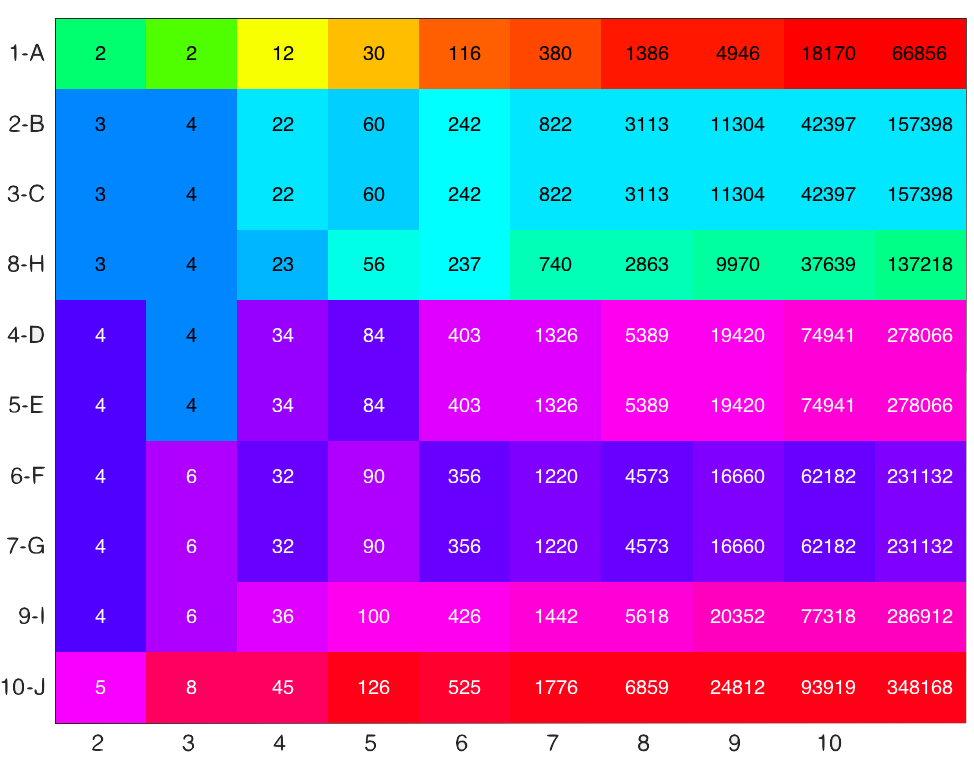
\includegraphics[width=.7\textwidth]{cyclesdemocycles}
\end{figure}

\subsection{Invertibility}
Note that if two graphs agree on the Cycles invariant, their complements (or inverses) likely agree on the Cycles invariant, but there is no proven reason to believe this is universally true.
The existence of non-isomorphic, co-cycles graphs raises the question: are their inverses necessarily co-cycles?
For all co-cycles graphs that were found, invertibility holds, but that is not a proof that it always holds.


\subsection{Time Complexity}
The running time of the paths invariant is the same whether we treat it as a vertex invariant or as a graph invariant.
The one difference is whether or not we sort the resulting vectors.
It is imperative to calculate $A^P$ even if we are only interested in calculating it for a single vertex.
Matrix multiplication can generally be accomplished in sub-cubic time CITE, but for the sake of simplicity and comprehensibility within this paper we will assume that it is an algorithm that runs in $O(N^3)$  time.
This means that the computation of any paths invariant can be accomplished in $O(N^4)$ time.
Though this sounds like a lot of time, in practice this is a fast computation.
It is made asymptotically better by the fact that efficient algorithms for matrix multiplication are well studied and optimized for a variety of contexts.
Matrix multiplication can be done efficiently by GPU arrays, and there are quick algorithms to do multiplication on sparse matrices for larger graphs.


\subsection{Operating over Large Numbers}
One element of the Cycles invariant that we will consistently need to be cognizant of is the fact that our numbers will grow very quickly, particularly for large values of N.
This complicates the calculation of cycles for values as small as $N=10$.
Integer overflow occurs when the summed value of the elements in the dot product add to a number greater than $2^{32}$ (on our system).
We can avoid this overflow if we guarantee that each of the $N$ pieces of the summation are less than or equal to $2^{\floor{32 - \log_2(N)}}$.
Since we arrive at each element in this dot-product-summation via the product of two elements that were previously somewhere in our running matrix, we can avoid an overflow in a computation step if we have:

$$ \forall_{i, j \in [1, N]} A[i, j] \leq \sqrt{2^{\floor{32 - \log_2(N)}}} = 2^{\floor{16 - 0.5\log_2(N)}}$$

We can make sure that this equality holds if we establish $K = \floor{16 - 0.5\log_2(N)}$ and make the incorporation of modulo into our formula for the Cycles function explicit:

$$ Cycles(A, v_i, p) = \begin{cases} 
      A[i,i] & p = 1 \\
      (Cycles(A, v_i, p-1) * A) \; \% \; 2^K  & p > 1
\end{cases}$$

This preserves the properties of addition and composition that we are looking for, and maintains reasonably sized bit arrays.
If we examine this methodology, we see that this operation is stable (if A and B map to the same value, they still will in this system) and that the odds of `collisions' (where values of A and B differ in the old system, and are the same in the new system) are unlikely.
The first claim is verified through the fact that if we break any integer $z_i$ into the portion of it divisible by $2^K$ ($x_i$), and the piece that is the remainder ($y_i$), then our properties of multiplication and addition hold under the modulo transformation (denoted $T_K(z_i)$) is stable/consistent:

$$z_i =  x_i(2^K) + y_i , \;\;\;T_K(z_i) = y_i$$

$$z_i + z_j = (x_i + x_j)(2^K) + (y_i + y_j)$$
$$T_K(z_i + z_j) = 0 + T_K(y_i + y_j)$$

$$z_i * z_j = (x_i*x_j)2^{2K} + (x_i*y_j + x_j*y_i)2^K + (y_i * y_j)$$
$$T_K(z_i * z_j) = 0 + 0 + T_K(y_i * y_j)$$

The second claim is verified through a thought experiment about how cycles varies over multiple values of $p$.
If we are attempting to distinguish between to cycles vectors, the most obvious comparison would be the degree of the vertices (the second element of a cycles vector).
If two vertices don't agree on this value, we have distinguished them successfully, and any future point of overlap (or collision) is irrelevant. 
If they agree on this value, then we know that each will have some minimum number of paths for any even value of p (as we know enough about their local neighborhood to assume the star graph as a minimum). 
Similarly, past values within the cycles invariant can be used to determine a large percentage of future values of the cycles invariant, for larger values of p.
The majority of the cycles described by the invariant are products of smaller cycles, so the `rate' at which they are added is highly correlated to past events.
To have a large number of newly emergent cycles in one but not the other (a precise enough one to exactly match the threshold for modulo) is incredibly unlikely.

Consider this argument by an analogy, one used to catch cheaters (people who cut courses) in looped Marathons and long track races.
If two people are in a race, and their first many splits are at the same times, it is very unlikely (even impossible) that one will lap the other over the course of a single split.
The same logic can be applied to think about the way that the number of closed cycles grows as $p$ grows.


\subsection{Space Complexity}
Though the above simplification can certainly allow us to do our computations in a way that is likely to avoid collisions, if we are discussing properties of the invariant as a whole, our analysis ignores the nature of collisions.
Thus, if we are attempting to draw conclusions about the algorithm from a theoretical perspective, we need to assume that we are fully calculating the cycles invariant without the use of the modulo trick.
This means that we need to prove that computation of it can be done in polynomial space.
Otherwise, the polynomial aspect of this computation could be misleading away from a gross inefficiency in space that masks the the true costs and limitation of the computation.
For example, there is \href{http://www.github.com/gbdubs/bytes}{a cute algorithm that I designed}, which solves the boolean satisfiability problem (an NPC-problem) in linear time, using only addition, multiplication and bitwise operations, but uses exponential space to do it. 
The flaw in this kind of algorithm is that it exploits a simplification that we make in algorithmic theory: we don't consider the time complexity on a bit-by-bit basis.
With large enough numbers, algebraic operations are not constant, they are linear functions of the number of their bits.
Infinitely sized registers are an abstraction of well designed systems, but cannot exist.
Thus it is important for us to verify that the calculation of the cycles invariant uses a polynomial amount of space.

In the worst case, the largest value in the Cycles invariant will occur when we have a fully connected graph of size N.
In a fully connected graph, any sequence of vertices that does not put the same vertex adjacent to itself is a valid cycle.
Thus, for a length $l$, there are exactly $(N-1)^l$ valid paths, of which exactly $(N-1)^{(l-1)}$ of which start and end at the same location (and thus are cycles).

If we assume that the maximum length cycle we are interested in is of length N-1 (as is discussed in another chapter), then the number bits required to express an individual number within the Cycles matrix is at maximum:
$$ O(Bits(N)) = O\Big( \log_2 \big[(N-1)^{N-1}\big] \Big) = O \big( (N - 1) * \log_2 [N-1] \big) = O(N \log_2 N)$$
Thus the total number of bits required to fully represent a Cycles matrix is bounded by $O(N^3logN)$, a large upper bound, but certainly sub-exponential.


\section{Reconstructability, Determination}
Many of the graph theoretic discussions of the cycles invariant will describe it with respect to other invariants. We have some language to assist these comparisons.
We will say that a property of a graph is `reconstructable' from Cycles if we can construct a valid value for the property if we are given the Cycles invariant of the graph.
Similarly, a property is determined by Cycles if a given value of the invariant allows exactly zero or one values for the property in question.
Reconstructability and determinability differ only in that reconstructability describes a procedure for the conversion, but doesn't guarantee a unique result, while determinability demands that a value for Cycles uniquely determines the property in question, but doesn't require us to show a technique by which to perform the determination.